This chapter describes the implementation of the cached profiles implementation for Hotspot, written as part of this thesis.
\\\\
Hotspot is an Java virtual machine implementation maintained by Oracle Corporation. It is part of the open source project \texttt{OpenJDK} and the source code is available at \url{http://openjdk.java.net/}.
\\\\
Most of the work is included in two new classes \texttt{/share/vm/ci/ciCacheProfiles.cpp} and \\\texttt{/share/vm/ci/ciCacheProfilesBroker.cpp} as well as modifications to \texttt{/share/vm/ci/ciEnv.cpp} and \texttt{/share/vm/compiler/compileBroker.cpp}.
\\
Most of the code is located in \texttt{/share/vm/ci/ciCacheProfiles.cpp}, a class that takes care of setting up a datastructure for the cached profiles as well as providing public methods to check if a method is cached or not. The class \texttt{/share/vm/ci/ciCacheProfilesBroker.cpp} gets called before a method that has a profile available gets compiled. It is responsible for setting up the compilation environment so the JIT compiler can use the cached profiles.
\\\\
A full list of modified files and the changes can be seen in the webrev or appendix TODO.
\\\\
The changes are provided in form of a patch for Hotspot version 8182 TODO. This original version is referred to as \textit{Baseline}.
\\\\
I will describe and explain the functionality and the implementation design decision in the following sections, ordered by the appearance in execution.


\section{Creating cached profiles}
\label{s:creatingprofiles}
The baseline version of Hotspot already offered a functionality to replay a compilation based on dumped profiling information.
This is mainly used in case the JVM crashes during JIT compilation to replay the compilation again and help finding the cause of this crash.
Dumping the data needed for the replay is either be done automatically in case of a crash or can be invoked manually by specifying the \texttt{DumpReplay} compile command option per method.
I introduce method option called \texttt{DumpProfile} as well as a compiler flag \texttt{-XX:+DumpProfiles} that appends profiling information to a file as soon as a method gets compiled. The first option can be specified as part of the \texttt{-XX:CompileCommand} or \texttt{-XX:CompileCommandFile} flag and allows one to select single methods to dump their profile. The second commands dumps profiles of all compiled methods into a single file.
The file can be opened with any text editor and is called \textit{cached\_profiles.dat}.
\\\\
As soon as a method gets compiled on level 3 or level 4 all information about the methods used in the compiled method as well as their profiling information get converted to a string and written to disk. Methods compiled with level 1 and 2 will not be considered. Both are rarely used in practice and do only include none respectively little profiling information.
\\\\
Since method often get compiled multiple times and at different tier, this can result in dumping compilation information about the same method multiple times. How this will be taken care of is described in Section \ref{s:initializingprofiles}.
Together with some additional information about the compilation itself, for example the bytecode index of the compiled method in case of OSR, the compiler will be able to redo the same compilation on a future run of the java virtual machine.  
\section{Initializing cached profiles}
\label{s:initializingprofiles}
I introduce a new compiler flag \texttt{-XX:+CacheProfiles} that enables the use of profiles that have been written to disk in a previous run of the Java Virtual Machine. Per default it reads from a file called \textit{cached\_profiles.dat} but a different file can be specified using \\\texttt{-XX:CacheProfilesFile=other\_file.dat}.
\\\\
Before any cached profiles can be used the virtual machine has to parse that file and organize the profiles and compile information in a simple datastructure. This datastructure is kept in memory during the whole execution of the JVM to avoid multiple scans of the file.
The parsing process gets invoked during boot up of the JVM, directly after the compileBroker gets initialized. This happens before any methods get executed and blocks the JVM until finished.
As mentioned in Section \ref{s:creatingprofiles} the file consists of method informations, method profiles and additional compile information. The parser scans the file once and creates a so called \texttt{CompileRecord} for each of the methods that include compilation information in the file. This compile record also includes the list of method information and their profiling information.
A method's compile information could have been dumped multiple times, so it can happen that there are multiple CompileRecords for the same method. In this case, Hotspot will only keep the CompileRecords that are created based on the last data written to the file.
Since profiling information only grow, the compilation that happened last contains the richest profile and is considered the best.
This is based on the fact that the richer the profile the more information about the method execution is known and influences the compiled version of that method. For example, a profile for a method might include data for all its branches and therefore no branches with uncommon traps which result in costly deoptimizations.
\\\\
The CompileRecord as well as the lists of methods information and profiles are implemented as an array located in Hotspot's heap space.
They get initialized with a length of 8 and grow when needed. The choice has been done for simplicity and leaves up room for further optimizations.

\section{Using cached profiles}
\label{s:usingprofiles}
The idea is to use cached profiles whenever possible and if none are available continue as usual.
\\\\
The thesis offers three different modes \texttt{mode0}, \texttt{mode1} and \texttt{mode2} on how the profiles are used.
The following paragraph describes the behaviour of mode0 and mode1 and I will discuss the differences in detail in Section \ref{s:cacheprofilesmode}, especially \texttt{mode2} in Section \ref{s:mode2}.

A graphical, simplified overview of the program flow for compiling a method with the changes introduced in this thesis can be found in Figure \ref{f:programflow}.
\begin{figure}[h]
  \begin{center}
    \centering
    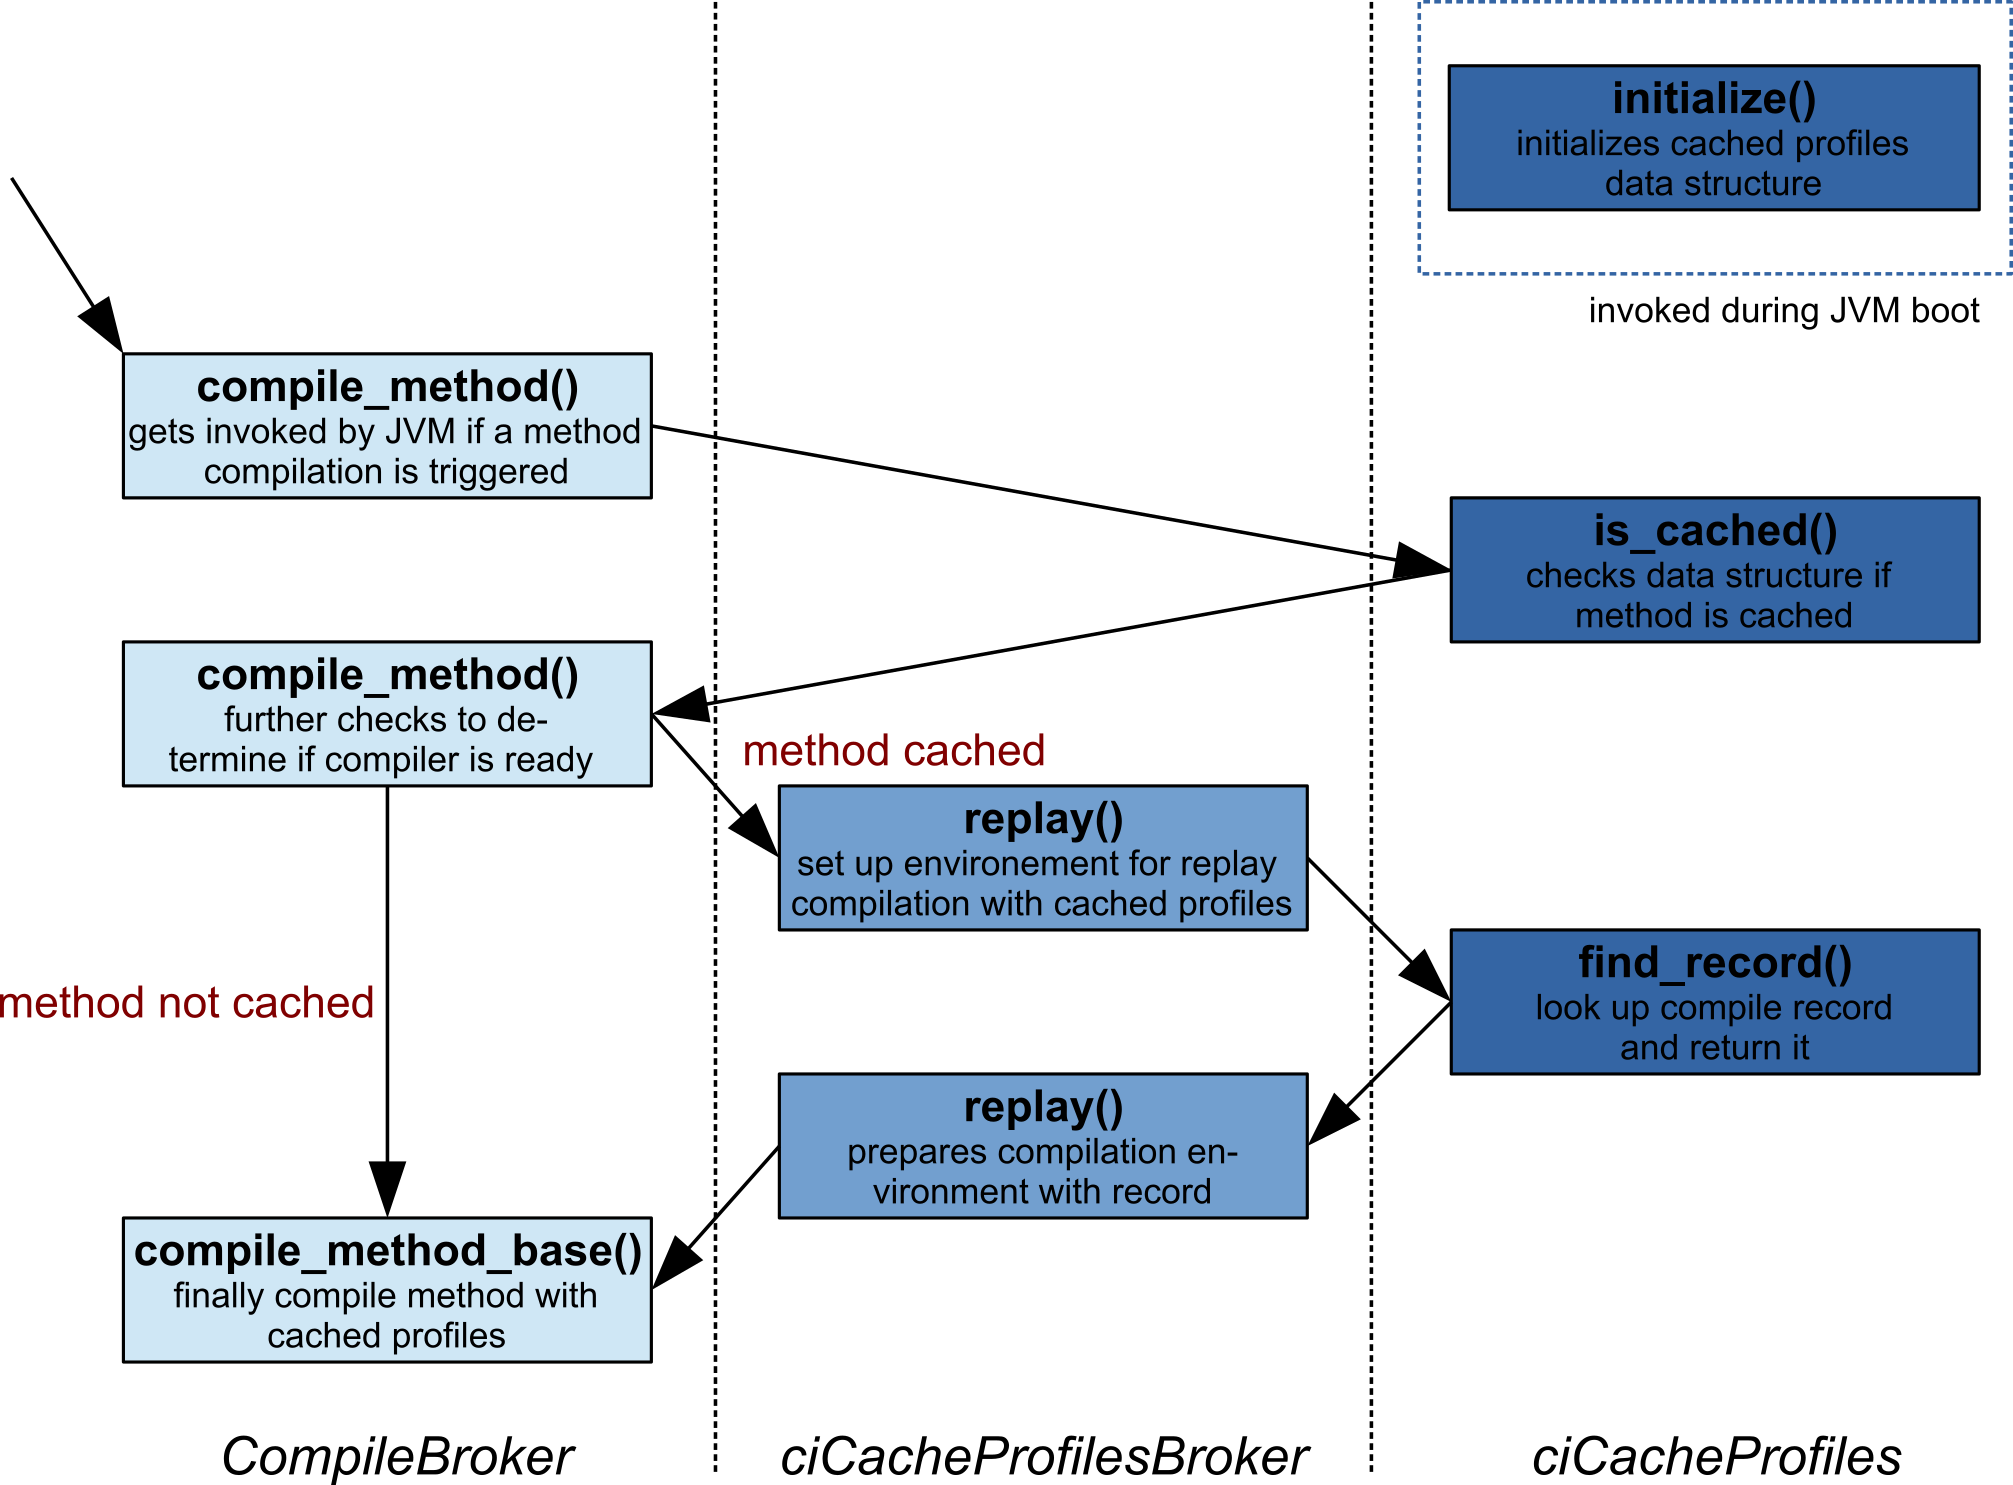
\includegraphics[width=0.8\textwidth]{figures/program_flow.png}
    \caption{program flow for compiling a method}
    \label{f:programflow}
  \end{center}
\end{figure}
As mentioned before once certain thresholds are exceeded a method gets scheduled for compilation. This means that the JVM will invoke a method called \texttt{compile\_method()} located in the \texttt{compileBroker} class. This method for example checks if the compile queue isn't full or if there is already another compilation of that particular method running.
I extended this method with a call to \texttt{ciCacheProfiles::is\_cached(Method* method)} which either returns 0 if the method is not cached or returns an integer value, reflecting the compile level, in case that method has a cached profile available. Because only methods compiled with level 3 or 4 get cached, this call only gets executed if the compilation request is also of level 3 or higher.
Note that this also means that if a method compilation of level 3 is initiated and a CompileRecord of level 4 is available that the highest level profile will be used. Therefore the method gets immediately compiled with C2 instead of C1.
In case the method is not cached the execution continues like in the baseline version.
Otherwise, the \texttt{compileBroker} calls into \texttt{ciCacheProfilesBroker} to replay the compilation, based on the saved profile.
The \texttt{ciCacheProfilesBroker} class then initializes the replay environment and retrieves the compile record from \texttt{ciCacheProfiles}. Subsequently the needed cached profiles get loaded to make sure they get used by a following compilation. ciCacheProfilesBroker then returns the execution to the compileBroker which continues with the steps needed to compile the method. Again some constraints are checked (e.g. if there is another compilation of the same method finished in the meantime) and a new compile job is added to the compile queue. Eventually the the method is going to be compiled using the cached profiles.
\\\\
Since the implementation is basically an extension of the static class \texttt{compileBroker}, \texttt{ciCacheProfiles} and \texttt{ciCacheProfilesBroker} are static classes as well. The \texttt{compileBroker} gets invoked by the single JVM main thread and is not multi threaded, therefore there is no need to make the compileRecord datastructure or any of the new implementations thread safe. 

\section{Different usage modes for cached profiles}
The implementation of cached profiles offers 3 different modes which differ in the transitions between the compilation tiers.
The motivation as well as the advantages and disadvantages of each mode are described in the following three subsections.
While \texttt{mode0} and \texttt{mode1} are similar except for the compile thresholds, \texttt{mode2} differs significantly.

\label{s:cacheprofilesmode}
\subsection{Compile Thresholds lowered (mode 0)}
\label{s:mode0}
The first mode is based on the consideration that a method that has a profile available does not require extensive profiling anymore. Therefore the compile thresholds (see Section \ref{s:compilethresholds}) of these methods are lowered automatically. By default, they are lowered to 1\% of their original values but the threshold scaling can be modified with the JVM parameter: \\\texttt{-XX:CacheProfilesMode0ThresholdScaling=x.xx}. 
\\1\% results in the level 3 invocation counter being reduced from 200 to 2. This means that the method will be interpreted once but then directly trigger a compilation on the next invocation.
Since the interpreter also handles class loading this decision has been made to avoid the need of doing class loading in C1 or C2 which was considered out of the scope for this thesis.
As mentioned before the triggered compilation will use the latest available compile record. Eventually, most hot methods get compiled by C2 and therefore the used compiled record is usually a C2 one. In this case the JVM will jump directly from compile level 0 to compile level 4 and avoid a costly C1 compilation as well as gathering profiling information during level 0 and level 3.
It will directly use the highly optimized version generated by C2 and ideally result in a lower time to reach peak performance.
On the downside this increases the load on the C2 compiler and fill the compile queue more quickly.
Mode 0 is the default mode and used if not further specified.
\subsection{Unmodified Compile Thresholds (mode 1)}
\label{s:mode1}
Mode 1 is doing exactly the same as mode 1 but does not scale the compilation thresholds automatically.
This is done to decrease the load increase on C2 as mentioned in Subsection \ref{s:mode0}.
Apart from this change mode 1 has the same behaviour as mode 0.
\subsection{Modified C1 stage (mode 2)}
\label{s:mode2}
Both modes mentioned before use cached profiles as soon as a compilation of level 3 and 4 are triggered. Since the thresholds for level 3 are smaller than the level 4 thresholds (see Appendix \ref{a:compilethresholds}) a method reaching a level 3 threshold could actually trigger a level 4 compilation, if the cached profile is one of level 4. So even if mode 1 is used and the thresholds are untouched C2 might get overloaded since compilations occur earlier.
\\\\
Mode 2 has been designed to make as little changes as possible to the tiered compilation. and prevent C2 being more used than usual. It does so by keeping the original tiered compilation steps and compilation thresholds and compiles methods with C1 prior to C2. But since there are already profiles available there is no need to run at Tier 3 to generate full profiles but instead it uses Tier 2.
Tier 2 does the same optimizations but offers only limited profiles like method invocation and backbranch counters. They are needed to know when to trigger the C2 compilation and therefore we can not use Tier 1. Tier 2 generally is considered about 30\% faster than Tier 3 \cite{code_atp_hpp}.
\\\\
If then the Tier4 thresholds are reached the method is compiled using C2 and the cached profiles.
\\\\
The above only makes sense if there is a C2 profile available.
If only a C1 profile is available, mode 2 will only use the profile during the C1 compilation and then use the new profiles.

\begin{figure}[h]
  \begin{center}
    \centering
    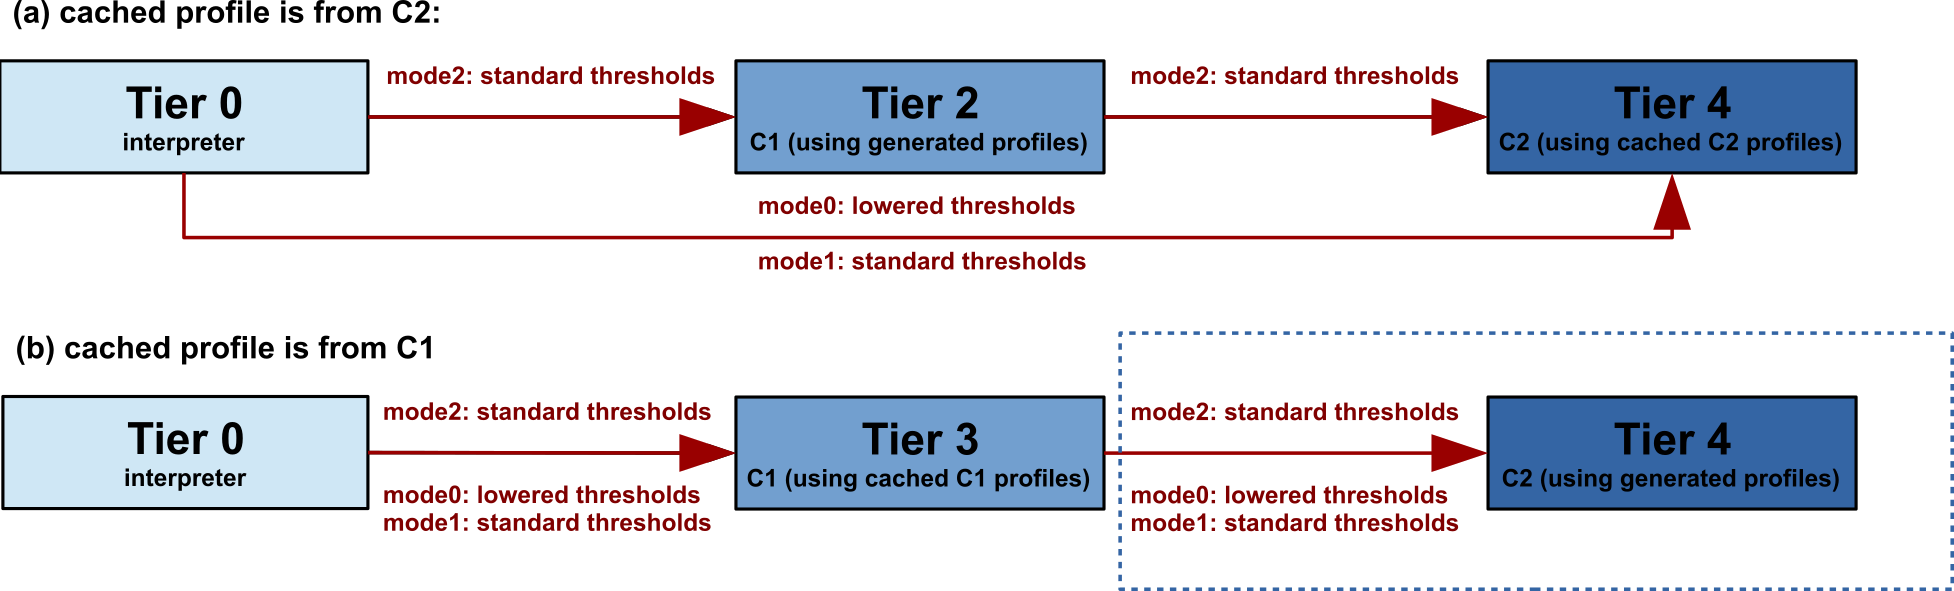
\includegraphics{figures/hs_tiers_threshold.png}
    \caption{Tier transitions of different modes}
    \label{f:hs_tiers_thresholds}
  \end{center}
\end{figure}


\section{Issues}
\label{s:issues}
If the profiles generated by multiple runs of the program deviate sharply it is likely that a cached profile does not fit to the current execution. In this case the compiled version would still trigger many deoptimizations and the method could end up having even worse performance since it's going to use the profile over and over again.
To circumvent that behavior I modified the code that only methods which have been deoptimized less then 10 times already will get compiled using cached profiles. If they are above that limit a standard compilation will be used instead.
The limit is 10 to allow a small number of recompilations. This could for example be useful when the method is deoptimized due to classes not being loaded. 
\\\\

\section{Debug output}
\label{s:debugoutput}
For debugging and benchmarking purposes I implemented four debug flags that can be used along with \texttt{-XX:+CacheProfiles}.
\begin{table}[ht]
  \centering
 % \caption{}
  \label{t:debugflags}
  \begin{center}
    \begin{tabular}{| l | p{9.0cm} |}
       \hline
       \textbf{flag} & \textbf{description} \\ \hline\hline
       -XX:+PrintCacheProfiles & enable command line debug output for cached profiles\\ \hline
       -XX:+PrintDeoptimizationCount & prints amount of deoptimizations when the JVM gets shut down\\ \hline
       -XX:+PrintDeoptimizationCountVerbose & prints total the amount of deoptimizations on each deoptimization\\ \hline
       -XX:+PrintCompileQueue & prints the total amount of methods in the compile queue each time a method gets added \\ \hline
    \end{tabular}
  \end{center}
\end{table}

 
